% Second draft, 29 Oct 2026 (after the independent code review and the rerun of Stages 3-4).
% Build: cd paper && xelatex main && xelatex main
% Figures come from ../results (python run_figures.py). Bibliography checked 30 Oct 2026 against publisher/repository pages.
\documentclass[11pt,a4paper]{article}
\usepackage{fontspec}
\setmainfont{Latin Modern Roman}
\setmonofont{Latin Modern Mono}
\usepackage[margin=2.4cm]{geometry}
\usepackage{amsmath,amssymb,bm}
\usepackage{graphicx}
\usepackage{booktabs,tabularx,multirow,array}
\usepackage[numbers,sort&compress]{natbib}
\usepackage{xcolor}
\usepackage[hidelinks]{hyperref}
\usepackage{caption}
\captionsetup{font=small,labelfont=bf}
\graphicspath{{../results/}}
\newcommand{\vect}[1]{\bm{#1}}
\newcommand{\todo}[1]{\textcolor{red}{[#1]}}
\setlength{\parskip}{3pt}

\title{Adaptive Augmentation of Incremental Nonlinear Dynamic Inversion under Rotor Faults:\\
A Fair Comparison of RLS, MRAC and $\mathcal{L}_1$ from Quadrotor to Quadplane}
\author{Azer Valizada\thanks{M.Sc.\ student, Mechanical Engineering, Technical University of Munich. \todo{contact}}}
\date{Draft, 29 October 2026}

\begin{document}
\maketitle

\begin{abstract}
Incremental nonlinear dynamic inversion (INDI) replaces most model knowledge with measured angular acceleration and keeps
a single model term, the control-effectiveness matrix. A rotor fault corrupts exactly this term. We compare three adaptive
augmentations of INDI, recursive least squares (RLS), predictor-based model-reference adaptive control (MRAC) and
$\mathcal{L}_1$ adaptive augmentation, under one protocol: the same plants, scenarios and metrics, fixed before any
adaptive method was run, and one tuning rule applied to each method on a separate scenario set. On a quadrotor,
$\mathcal{L}_1$ closes 183\,\% of the gap between baseline INDI and an INDI that knows the fault (RLS 153\,\%, MRAC 87\,\%).
On a 5\,kg quadplane flying at 0--12\,m/s, with weighted least-squares allocation over rotors and control surfaces,
$\mathcal{L}_1$ closes 145\,\%, RLS 106\,\% and MRAC 63\,\% (81\,\% on the scenarios every method survives). Two design details decide the estimators. RLS must remove the wing's
known contribution from its measurement, and its estimate must be bounded away from zero: an estimate at zero removes the rotor
from the allocation and thereby from its own data. Even then RLS does not identify the fault: its estimate freezes at a wrong value,
yet control stays good. MRAC needs the aerodynamic model, and with an unknown wind its estimates drift even
without a fault. $\mathcal{L}_1$ is also best under gusts, doubled sensor noise, a slower motor and a wrong aerodynamic model. Its price
is the delay margin: 18\,ms on the quadrotor and 20\,ms on the quadplane, against 25 and 45\,ms for the other methods. A one-axis linear
model reproduces these margins and shows that $\mathcal{L}_1$ doubles the inner-loop crossover frequency. On the quadplane, the
complete loss of a lift rotor can be recovered from 6--8\,m/s. A controller-independent trim analysis gives the same limit under
pitch and heading hold, so no adaptive method moves it by more than 1\,m/s. If the rotor fails during the transition, continuing to
accelerate lets the aircraft complete it after a loss at 4\,m/s in most cases.
\end{abstract}

% =====================================================================================================
\section{Introduction}
Incremental nonlinear dynamic inversion computes the actuator command as an increment on the current, measured
state: the unknown part of the dynamics is contained in the measured angular acceleration, and only the control
effectiveness $G$ must be known \cite{sieberling2010,smeur2016}. This makes INDI robust to aerodynamic and inertial model
errors and has made it popular for multirotors and hybrid aircraft \cite{smeur2016,sun2020,deponti2023}. A rotor fault,
for example a damaged propeller, is different: it changes $G$ itself. The controller then still converges, because
every residual error is measured again at the next step, but it does so more slowly, and the attitude transient grows.

Three families of methods restore performance by adapting the controller online. Least-squares estimation of the
effectiveness from INDI's own increments was proposed by Smeur et al.~\cite{smeur2016}. Predictor-based MRAC estimates the same
quantities with a Lyapunov-derived law and has been used for adaptive control allocation \cite{falconi2021,franceschini2026}.
$\mathcal{L}_1$ adaptive augmentation estimates a lumped uncertainty and cancels a low-pass-filtered copy of it
\cite{hovakimyan2010,raos2026,mao2023}. Each has been shown on its own vehicle, tuned by its authors. For quadplanes,
Wang and Sun~\cite{wang2021} handle the complete loss of a rotor with incremental adaptive sliding-mode control, Cai and Lovera~\cite{cai2025} reallocate
rotors and surfaces during the transition with fault information assumed known, and Fu et al.~\cite{fu2025} design an adaptive
fault-tolerant attitude controller for the transition. We found no study that compares RLS, MRAC and $\mathcal{L}_1$ on INDI
under one protocol, none that follows them from a quadrotor to an over-actuated quadplane, and none that reports the minimum
airspeed at which a quadplane survives a lift-rotor fault. \todo{literature check of 28 Oct used abstracts only; read full texts}

\paragraph{Contributions.}
\begin{enumerate}
\item A comparison fixed in advance: scenarios and metrics were set before any adaptive method ran on a vehicle, every
  method was tuned on a separate scenario set with the same rule, and every later rule change was logged with its reason.
\item The same three methods on two very different vehicles, including robustness measures that headline results
  usually omit: false fault detection under gusts and the margin against an unmodelled actuator delay.
\item A linear explanation of the delay sensitivity of $\mathcal{L}_1$-augmented INDI, which reproduces the simulated margins.
\item Two failure modes of estimation-based adaptation in over-actuated INDI: an effectiveness estimate that reaches zero removes
  its actuator from the allocation and locks itself, and a model-based estimator that confuses ground and air velocity drifts in wind.
\item For the quadplane, the minimum safe airspeed after a lift-rotor fault, checked against a controller-independent trim
  analysis, and the finding that continuing the transition outruns faults that cannot be recovered at constant speed.
\end{enumerate}
The simulation, tests and every script that produces a number in this paper are open \todo{repository link}.

% =====================================================================================================
\section{Vehicles and fault model}
\subsection{Quadrotor}
A 1\,kg X-quadrotor with $J = \mathrm{diag}(0.0089, 0.0089, 0.016)$\,kg\,m$^2$, arm 0.17\,m, yaw-torque coefficient
$k_m = 0.016$\,m, maximum rotor thrust 6\,N and first-order motors with $\tau_m = 20$\,ms. The rigid-body equations
(Newton--Euler, quaternion attitude) are integrated with fourth-order Runge--Kutta at 1\,ms; the controller runs at 500\,Hz.
The gyro (0.002\,rad/s) and accelerometer (0.05\,m/s$^2$) are noisy; position, velocity and attitude are measured without noise.

\subsection{Quadplane}
The quadplane follows the PX4 \texttt{standard\_vtol} model \cite{px4models}: 5\,kg, $J = \mathrm{diag}(0.478, 0.342, 0.811)$\,kg\,m$^2$,
four lift rotors at $(\pm0.35, \pm0.35)$\,m, a pusher on the axis, ailerons and an elevator, wing area $S = 1.0$\,m$^2$ and span
$b = 2.144$\,m. The aerodynamic coefficients are the non-dimensional Aerosonde set of Beard and McLain~\cite{beard2012} applied to this geometry,
with a flat-plate blend beyond stall for lift, drag and the pitching moment (beyond stall the flat-plate normal force $2\sin\alpha$ acts at
the linear static margin, so $C_m$ is continuous for all $\alpha$); the sideslip terms saturate at $30^\circ$. All forces and moments scale with the dynamic pressure $\bar q = \tfrac12\rho V_a^2$:
\begin{equation}
L = \bar q S b\, C_\ell,\qquad M = \bar q S c\, C_m,\qquad N = \bar q S b\, C_n,
\end{equation}
with linear stability, damping and control derivatives (e.g.\ $C_m = C_{m_0} + C_{m_\alpha}\alpha + C_{m_q}\tfrac{c}{2V_a}q + C_{m_{\delta_e}}\delta_e$).
We deviate from PX4 where its values would make faults trivial or the aerodynamics unrealistic (Table~\ref{tab:qp}).
The aileron's roll authority exceeds the rotors' ($\approx 8.6$\,Nm) at 9--10\,m/s; at 15\,m/s the wing carries 65\,\% of the
weight. A pitot tube measures airspeed (0.2\,m/s noise); servo positions are not measured.

\begin{table}[t]
\centering\small
\caption{Quadplane: deviations from the PX4 \texttt{standard\_vtol} model and their reasons.}
\label{tab:qp}
\begin{tabularx}{\linewidth}{>{\raggedright\arraybackslash}p{3.2cm} >{\raggedright\arraybackslash}p{2.3cm} >{\raggedright\arraybackslash}p{2.6cm} >{\raggedright\arraybackslash}X}
\toprule
Quantity & PX4 & Here & Reason\\
\midrule
max.\ lift-rotor thrust & 45\,N & 24.5\,N & PX4 gives thrust/weight 3.7, at which faults are trivial; lift systems are sized near 2\\
yaw torque per thrust $k_m$ & 0.06\,m & 0.025\,m & estimated for a 15-inch propeller, $D\,C_Q/C_T$\\
max.\ pusher thrust & 105\,N & 20\,N & cruise drag at 15\,m/s is $\approx$7\,N\\
surface limit & $\pm45^\circ$ & $\pm25^\circ$ & linear coefficients are not credible beyond $\approx25^\circ$\\
servo dynamics & -- & first order, 30\,ms & not in PX4\\
aerodynamics & one $C_L$ slope per half wing & full coefficient set \cite{beard2012} & PX4 plug-in has no control or damping derivatives\\
\bottomrule
\end{tabularx}
\end{table}

\subsection{Fault model}
Rotor $i$ produces $\eta_i T_i$, where $T_i$ is the thrust a healthy rotor would produce at its current speed; $\eta_i = 1$
is healthy and $\eta_i = 0$ a lost propeller. The rpm-based thrust measurement cannot see $\eta_i$; the gyro and the
accelerometer can. Faults are abrupt or 1\,s linear ramps.

% =====================================================================================================
\section{Control}
\subsection{Baseline INDI}
Position errors give a desired acceleration and thrust direction; the attitude error gives a rate command $\vect\omega_c$, and
the rate loop gives the desired angular acceleration $\vect\nu = K_\omega(\vect\omega_c - \vect\omega)$. Writing the rotational
dynamics as $\dot{\vect\omega} = \vect F(\vect x) + G\vect u$ and expanding around the current, measured state,
\begin{equation}
\dot{\vect\omega} \approx \dot{\vect\omega}_0 + G(\vect u - \vect u_0)
\quad\Rightarrow\quad
\vect u = \vect u_0 + G^{-1}(\vect\nu - \dot{\vect\omega}_0),
\label{eq:indi}
\end{equation}
where $\dot{\vect\omega}_0$ and $\vect u_0$ are the gyro derivative and the measured actuator state, passed through identical
second-order filters ($\omega_n = 50$\,rad/s, $\zeta = 0.55$) so that their increments refer to the same instant \cite{smeur2016}.
$\vect F$ cancels; only $G$ is needed. The total thrust is treated the same way, with the current thrust measured by the
accelerometer. (A thrust channel based on rotor speed instead loses $(mg/4)(1/\eta - 1)/(m k_{p,z})$ of altitude after a fault,
0.96\,m at $\eta = 0.5$; the simulation matches this within 3\,\%, and the accelerometer removes it, 0.003\,m. All comparisons use
the accelerometer-based baseline.)

After a fault the true effectiveness is $G\,\mathrm{diag}(\vect\eta)$, and one INDI step achieves only
$\dot{\vect\omega}_0 + G\,\mathrm{diag}(\vect\eta)\,G^{-1}(\vect\nu - \dot{\vect\omega}_0)$: the loop still converges, at a
lower effective gain. The \emph{oracle INDI} uses $G\,\mathrm{diag}(\vect\eta)$ with the true $\vect\eta$. It is a reference
for the value of fault knowledge, not an upper bound: a method that reacts harder can recover faster.

\subsection{Allocation on the quadplane}
On the quadplane four lift rotors and two surfaces produce three moments and the body-$z$ force, so $G(V_a)$ is
$4\times 6$ and its surface columns grow with $\bar q$. Equation~\eqref{eq:indi} is replaced by weighted least squares with
actuator limits,
\begin{equation}
\min_{\Delta\vect u}\ \gamma\,\|W_v(G\Delta\vect u - \vect v)\|^2 + \|W_u(\Delta\vect u - \Delta\vect u_p)\|^2
\quad\text{s.t.}\quad \vect u_{\min} - \vect u_0 \le \Delta\vect u \le \vect u_{\max} - \vect u_0,
\end{equation}
solved by the active-set method of H\"{a}rkeg\aa{}rd~\cite{harkegard2002} ($\gamma = 1000$, $W_v = \mathrm{diag}(1,1,0.3,0.3)$). Actuators are
normalised by their range and weighted equally; the preferred state (equal rotors, surfaces at zero) is approached with a 0.2\,s
time constant. No scheduling rule is needed: as $\bar q$ grows, the surfaces become the cheaper way to produce a moment and
take over the load. The pusher closes the forward-acceleration loop incrementally on the accelerometer, pitch is held at zero,
and the servo positions come from a first-order model in the controller.

\subsection{Adaptive augmentations}
All three plug into the same INDI core: RLS and MRAC replace $G$ by $G\,\mathrm{diag}(\hat{\vect\eta})$; $\mathcal{L}_1$
modifies $\vect\nu$.

\paragraph{Known non-rotor part.} On the quadplane the angular acceleration and the body-$z$ force also contain the wing (damping,
static stability, surfaces, lift), the pusher torque and the gyroscopic term. RLS and MRAC receive the same nominal model of this part,
computed from the measured velocity, attitude, rates and the servo model, with ground velocity taken as air velocity:
$\vect o = \big[J^{-1}(\vect M_\text{aero} + \vect M_\text{push} - \vect\omega\times J\vect\omega);\ -F_{z,\text{aero}}\big]$, passed through the
same synchronisation filter ($\vect o_f$). $\mathcal{L}_1$ uses no model of it.

\paragraph{RLS.} Over $L$ control steps, INDI's own linearisation gives a measurement equation linear in $\vect\eta$,
\begin{equation}
\vect y = \Delta\left(\begin{bmatrix}\dot{\vect\omega}_f\\ -m a_{z,f}\end{bmatrix} - \vect o_f\right)
= G_\text{rot}\,\mathrm{diag}(\Delta\vect u_f)\,\vect\eta = \Phi\vect\eta,
\end{equation}
solved recursively with forgetting factor $\lambda$, rows weighted by their measured noise, a dead-zone on $\|\Delta\vect u_f\|$
against closed-loop bias, and $\hat{\vect\eta}$ clipped to $[\eta_{\min}, 1.5]$; $\vect o$ is zero on the quadrotor. On noise-free
data, batch least squares on these rows returns the true $\vect\eta$ at 0, 8 and 12\,m/s (a regression test).

\paragraph{MRAC.} A predictor of the rotational dynamics runs beside the vehicle,
$\dot{\hat{\vect\omega}} = J^{-1}B\,\mathrm{diag}(\hat{\vect\eta})\vect T + \vect o_{1:3} - a(\hat{\vect\omega}-\vect\omega)$,
and the Lyapunov function $V = \tfrac12\vect e^\top\vect e + \tfrac12\tilde{\vect\eta}^\top\Gamma^{-1}\tilde{\vect\eta}$ gives
$\dot{\hat{\vect\eta}} = -\Gamma\,\mathrm{diag}(\vect T)\,(J^{-1}B)^\top\vect e$ with $\dot V = -a\vect e^\top\vect e$; a gradient term
on the accelerometer-measured thrust (minus the filtered nominal lift) is added.

\paragraph{$\mathcal{L}_1$.} With $\dot{\vect\omega} \approx A(s)[\vect\nu_a] + \vect\sigma$, $A(s)$ the motor lag and $\vect\sigma$
everything INDI misses, a state predictor
$\dot{\hat{\vect\omega}} = -a(\hat{\vect\omega}-\vect\omega) + A(s)[\vect\nu_a] + \hat{\vect\sigma}$, the piecewise-constant law
\begin{equation}
\hat{\vect\sigma}_k = -\frac{e^{-aT_s}}{\Phi}\,(\hat{\vect\omega}_k - \vect\omega_k),\qquad \Phi = \frac{1 - e^{-aT_s}}{a},
\end{equation}
and the compensation $\vect\nu_a = \vect\nu - C(s)[\hat{\vect\sigma}]$ with $C(s) = \omega_c/(s+\omega_c)$ \cite{hovakimyan2010}.
$\mathcal{L}_1$ needs no model of the vehicle beyond the motor lag.

Both estimators start learning 0.5\,s after the filters are initialised. The lower bound $\eta_{\min}$ is 0.1 for RLS on both
vehicles and 0 for MRAC on the quadplane. For RLS on the quadplane it was first set to 0, before tuning, because the scenarios include complete
rotor loss; we changed it to 0.1 after seeing the results (Section~\ref{sec:lockin}), and report 0 as a sensitivity result.

% =====================================================================================================
\section{Evaluation protocol}
\paragraph{Scenarios.} Quadrotor: hover with position steps; a grid of 24 faults (4 rotors $\times$ $\eta\in\{0.8, 0.65, 0.5\}$
$\times$ abrupt / 1\,s ramp) and 100 Monte Carlo runs (random fault $\eta\sim U[0.5,0.9]$, mass $\pm5$\,\%, inertia $\pm10$\,\%, noise
seed). Quadplane: steady level flight at $V\in\{0,4,6,8,10,12\}$\,m/s with 4 rotors $\times$ $\eta\in\{0.6, 0.3, 0\}$ (72 runs);
a speed sweep 0--12\,m/s in 1\,m/s steps for $\eta\in\{0.3, 0.15, 0\}$; 100 Monte Carlo runs including $\pm20$\,\% error in the
surface effectiveness. Transition: hover, then 1, 2 or 3\,m/s$^2$ to 16\,m/s, with a front or rear rotor failing as the reference
passes $V_f\in\{0,2,\dots,12\}$\,m/s, $\eta\in\{0.3, 0\}$ (84 runs). Gust checks apply a 0.5\,s step moment to the healthy vehicle.

\paragraph{Metrics.} Quadrotor: peak attitude error in $[t_0, t_0 + t_\text{ramp} + 0.5\,\text{s}]$. The quadplane's inertia is about 50
times larger and its failures develop over seconds, so the window is 4\,s and the primary metric is the peak \emph{tilt} error,
the angle between the desired and actual body $z$ axes; heading is reported separately, because without a rudder a heading drift
is not by itself unsafe. Loss of control: divergence (including more than 100\,m from the reference), tilt above $90^\circ$, or more
than 5\,m altitude loss. Recovered: final tilt below $1^\circ$ and heading below $5^\circ$. The \emph{gap closed} is
$\sum(b - m)/\sum(b - o)$ over scenarios survived by all controllers, with $b$, $m$, $o$ the baseline, method and oracle values,
and a 95\,\% bootstrap interval (4000 resamples); method differences use a paired bootstrap.

\paragraph{Tuning.} Each method was tuned on a separate tuning set with one rule: lowest mean primary metric over the faulty
scenarios, subject to (a) no loss of control, (b) fault-free attitude RMS at most 1.05 times the baseline's (+0.01$^\circ$ on the
quadplane, whose noise floor is 0.002$^\circ$), and (c) healthy-rotor estimates within 0.15 of one. Rule (c) was added after the first
RLS run, where the best-scoring setting drove healthy estimates to the clip limit. Every method on both vehicles gets the same procedure and budget: a 48-candidate grid, then a local search of up to 48 more
candidates that steps one notch along each parameter's ordered ladder until no neighbour is better. Every winner is interior with all
neighbours evaluated, or at a physical bound (RLS $L = 1$ and $\lambda = 1$, MRAC $\gamma_d = 0$, $\mathcal{L}_1$ $\omega_c = 1280$\,rad/s near
the Nyquist rate of the 500\,Hz loop, and on the quadrotor the $a \to 0$ limit of $\mathcal{L}_1$). Where a first search ended on the
edge of a ladder that is not a physical bound (on the quadrotor, MRAC $\gamma_T$ and $\mathcal{L}_1$ $a$), the ladder was extended and
the method re-tuned. The procedure is the same, but not every aspect is symmetric. $\mathcal{L}_1$ has two parameters, so its 48 grid points
form a $4\times12$ grid, finer per axis than the $3\times4\times2\times2$ of RLS and MRAC. Rule (c) binds only on the estimators; without it
RLS and MRAC would score better but drift by 0.9--1.0 in healthy flight. $\mathcal{L}_1$'s $\omega_c = 1280$\,rad/s passes 92\,\% of a new
estimate per step, which is practically the unfiltered limit: the tuned $\mathcal{L}_1$ acts as a predictor-based disturbance observer.
Some choices are ties within 0.1\,\% of the score (RLS $\lambda = 1$ against 0.999, MRAC $\gamma_d = 0$ against 3). The quadplane tuning set
is small: four partial faults at 2--11\,m/s and one fault-free run, without hover, complete loss or wind.

\paragraph{Independent reviews.} Before the final runs, two blind reviews of the code (by separate agents that had not seen it being
written) were carried out. The first found two critical and seven major problems in the quadplane part, among them the incomplete RLS
measurement model above, an unbounded pitching moment at large angles, and a per-speed table that averaged each controller over its own
survivors. The second found no critical problem; its major findings were a wing force that changed sign in pure sideways flow (lift,
drag and pitch moment now use the dynamic pressure of the flow in the body $x$--$z$ plane), a post-stall moment that did not match the
post-stall force, the frozen RLS estimate (Section~\ref{sec:lockin}) and the tuning asymmetries above. After each review every quadplane and
transition result was re-tuned and rerun; the reviews, the fixes and their effect on each number are in the repository.

% =====================================================================================================
\section{Results: quadrotor}
\begin{table}[t]
\centering\small
\caption{Quadrotor. Mean peak attitude error, gap closed with 95\,\% bootstrap interval, gust response and delay margin. No run is lost.}
\label{tab:quad}
\resizebox{\linewidth}{!}{\begin{tabular}{lcccccc}
\toprule
 & Grid (24) & Monte Carlo (100) & Gap closed, grid / MC & Gust & False detection & Delay margin\\
\midrule
Baseline INDI & 1.60$^\circ$ & 1.27$^\circ$ & 0\,\% & 0.78$^\circ$ & -- & 25\,ms\\
RLS & 0.69$^\circ$ & 0.51$^\circ$ & 153 [132, 183] / 183 [170, 199]\,\% & 0.56$^\circ$ & 0.80 & 25\,ms\\
MRAC & 1.08$^\circ$ & 0.89$^\circ$ & 87 [84, 91] / 92 [89, 94]\,\% & 0.78$^\circ$ & 0.16 & 25\,ms\\
$\mathcal{L}_1$ & 0.50$^\circ$ & 0.44$^\circ$ & 183 [171, 206] / 200 [189, 212]\,\% & 0.34$^\circ$ & -- & 18\,ms\\
Oracle INDI & 1.00$^\circ$ & 0.86$^\circ$ & 100\,\% & 0.78$^\circ$ & -- & 25\,ms\\
\bottomrule
\end{tabular}}
\end{table}
Table~\ref{tab:quad} summarises the quadrotor (settings: RLS $L = 10$, threshold 0.005\,N, $\lambda = 0.97$, $p_0 = 0.3$; MRAC $a = 10$,
$\Gamma = 1$, $\gamma_T = 20$; $\mathcal{L}_1$ $a = 0.1$, $\omega_c = 1280$). All pairwise differences are significant (paired bootstrap, grid
and Monte Carlo). RLS and $\mathcal{L}_1$ beat the oracle
by reacting harder, at the cost of more motor saturation. RLS also reacts to gusts: the estimates of healthy rotors move by up to
0.80, a false fault detection, because its measurement model has no disturbance term and the least-squares fit explains the gust
with $\hat{\vect\eta}$. MRAC estimates more accurately (final error 0.10 against 0.14 for RLS) but adapts more slowly; raising its gain
produces a 13.5\,Hz oscillation between diagonal rotors, which the roll and pitch rows cannot tell apart. The tuned $\mathcal{L}_1$
($a = 0.1$\,s$^{-1}$, the $a \to 0$ limit where the score has converged, and $\omega_c = 1280$\,rad/s, near the Nyquist rate) oscillates with
20\,ms of unmodelled delay; with $a = 300$\,s$^{-1}$ it keeps the 25\,ms margin of the other methods (Section~\ref{sec:delay}).

% =====================================================================================================
\section{Results: quadplane at constant airspeed}
\subsection{Comparison}
\begin{table}[t]
\centering\small
\caption{Quadplane. Mean peak tilt over the grid scenarios (72 faults at 0--12\,m/s) and the Monte Carlo scenarios survived by all
controllers; gap closed with 95\,\% bootstrap interval over the scenarios that baseline, oracle and the method survive (common set of all
controllers in brackets); gust response (false detection: mean / worst estimate drift); delay margin in hover and at 8\,m/s. Losses: of 72 grid runs.}
\label{tab:qp_res}
\resizebox{\linewidth}{!}{\begin{tabular}{lccccccc}
\toprule
 & Lost & Grid tilt & Gap closed, grid & Gap closed, MC & Gust tilt & False detection & Delay margin\\
\midrule
Baseline INDI & 2 & 1.39$^\circ$ & 0\,\% & 0\,\% & 0.19$^\circ$ & -- & 45 / $\ge$60\,ms\\
RLS & 2 & 0.63$^\circ$ & 106 [100, 114] (112)\,\% & 109 [99, 120]\,\% & 0.16$^\circ$ & 0.42 / 0.71 & 45 / $\ge$60\,ms\\
MRAC & 2 & 0.84$^\circ$ & 63 [45, 81] (81)\,\% & 79 [67, 90]\,\% & 0.19$^\circ$ & 0.10 / 0.15 & 45 / $\ge$60\,ms\\
$\mathcal{L}_1$ & 6 & 0.39$^\circ$ & 145 [139, 153] (145)\,\% & 147 [128, 167]\,\% & 0.07$^\circ$ & -- & 20 / 20\,ms\\
Oracle INDI & 2 & 0.71$^\circ$ & 100\,\% & 100\,\% & 0.19$^\circ$ & -- & 45 / $\ge$60\,ms\\
\bottomrule
\end{tabular}}
\end{table}
Table~\ref{tab:qp_res} shows the quadplane results (RLS $L = 1$, threshold 0.05\,N, $\lambda = 1$, $p_0 = 0.01$, $\eta_{\min} = 0.1$;
MRAC $a = 30$, $\Gamma = 16$, $\gamma_T = 1$; $\mathcal{L}_1$ $a = 30$, $\omega_c = 1280$). The gap closed is taken over the scenarios
that baseline, oracle and the method all survive; on the common set of all controllers MRAC rises to 81\,\% and RLS to 112\,\%, and the
ranking is the same. $\mathcal{L}_1$ is again best, also under gusts, where it has no fault to misdiagnose: a gust is part of $\vect\sigma$
and cancelling it is correct. RLS matches the oracle; it reads a gust as a fault on all four rotors (estimates move by 0.42 on average and
0.71 at worst), so it fits an effectiveness to whatever the rotors did not deliver rather than identifying a fault
(Section~\ref{sec:lockin}). $\mathcal{L}_1$ has the lowest mean peak tilt at every airspeed, but its six losses are all complete rotor
losses at 0 and 4\,m/s, where the other controllers survive without recovering (Section~\ref{sec:minspeed}). Repeating the grid and the transition
grid with two further noise seeds changes each gap closed by at most 8 percentage points (RLS on the grid, 106--114\,\%) and leaves the ranking
unchanged; the losses differ in one run (one RLS grid loss fewer with one seed).

Figure~\ref{fig:alloc} shows how the allocation shares the load after rotor 1 drops to 30\,\%. Below 4\,m/s the damaged rotor and both
surfaces saturate and the heading is lost; above, the rotor commands even out and the surface deflection shrinks with $\bar q$.

\begin{figure}[t]
\centering
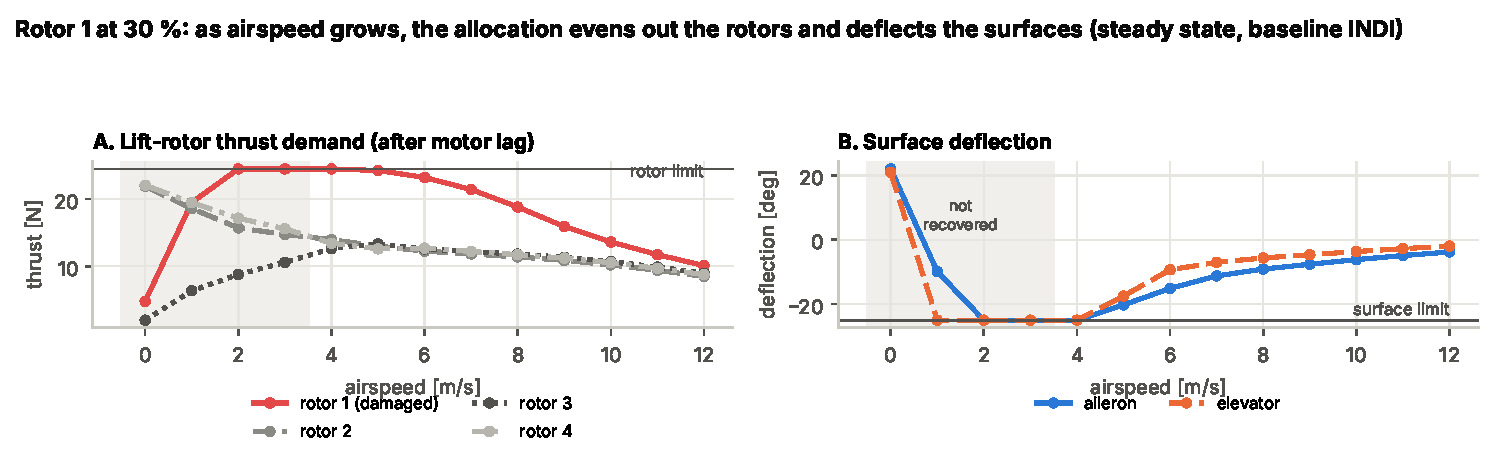
\includegraphics[width=0.85\linewidth]{fig2_allocation_vs_speed.pdf}
\caption{Steady state after rotor 1 drops to 30\,\%, baseline INDI. The allocation needs no scheduling rule: as dynamic pressure grows,
the surfaces take over and the rotors even out.}
\label{fig:alloc}
\end{figure}

\subsection{Minimum safe airspeed}\label{sec:minspeed}
\begin{figure}[t]
\centering
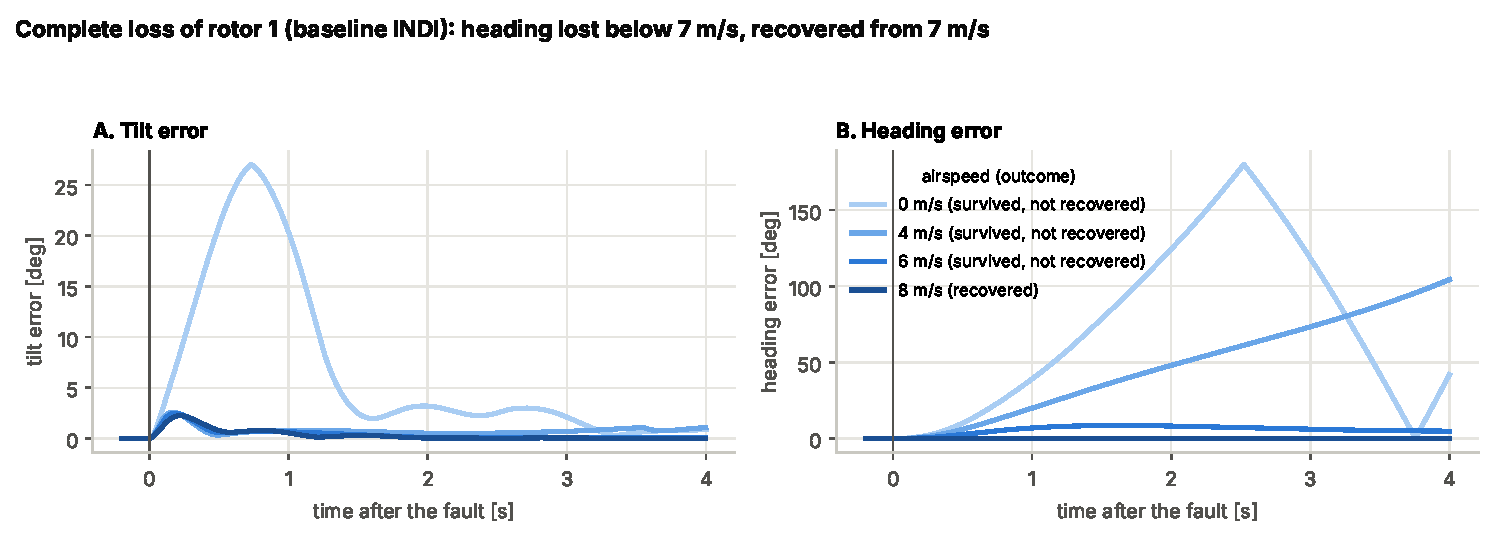
\includegraphics[width=0.85\linewidth]{fig1_rotor_loss_speed.pdf}
\caption{Complete loss of rotor 1 at constant airspeed, baseline INDI. In hover the aircraft stays upright on the two diagonal rotors
but spins; at 4\,m/s it keeps its tilt but loses heading; at 6\,m/s the heading error stays small but does not settle
within the tolerance; at 8\,m/s it recovers fully (limit: 7\,m/s).}
\label{fig:loss}
\end{figure}
Figure~\ref{fig:loss} shows the complete loss of a front rotor at four airspeeds. The lowest airspeed from which every faster one recovers
is 4 / 5\,m/s (front / rear rotor) for $\eta = 0.3$, 6 / 7\,m/s for $\eta = 0.15$ and 6--7 / 8\,m/s for a lost rotor. The five
controllers differ by at most 1\,m/s, with no consistent winner. In hover a complete loss is not recoverable by any controller. With a front
rotor lost, baseline, oracle, RLS and MRAC hold the altitude on the two diagonal rotors and give up yaw, the spinning mode known from
quadrotors \cite{mueller2014}; $\mathcal{L}_1$, which treats the yaw torque as a disturbance to cancel, is lost. With a rear rotor lost
every controller is lost in hover; at 4\,m/s all but $\mathcal{L}_1$ survive at 50--60$^\circ$ of tilt. These runs fly through large sideslip and
angles of attack, where the aerodynamic model is least trustworthy: the correction of the wing model after the second review changed which
of them count as lost. We read them as ``no controller recovers'', not as a ranking.

To see whether the limit is physical or set by the controller, we asked a controller-independent question: does a steady, straight, level
flight condition exist at that airspeed with the actuators within their limits? Solving the six force and moment balances and a level flight
path for rotor thrusts, deflections, pusher, angle of attack, sideslip and bank (bounded nonlinear least squares, eight starts) gives
Fig.~\ref{fig:feas}. Under the controller's constraints, pitch held and sideslip within $5^\circ$ (the heading criterion), the static limit
equals the simulated one for $\eta = 0.3$ and for a lost rear rotor, and lies within 0.5--1\,m/s of it otherwise (the simulation uses a 1\,m/s grid). Under these constraints the limit is
physical, which is why fault knowledge does not move it. Accepting 20$^\circ$ of sideslip lowers it by 1--1.5\,m/s, and a free pitch angle
further (complete loss: 4.5 / 4--4.5\,m/s): a recovery mode that trades heading and pitch for authority could extend the safe envelope.

\begin{figure}[t]
\centering
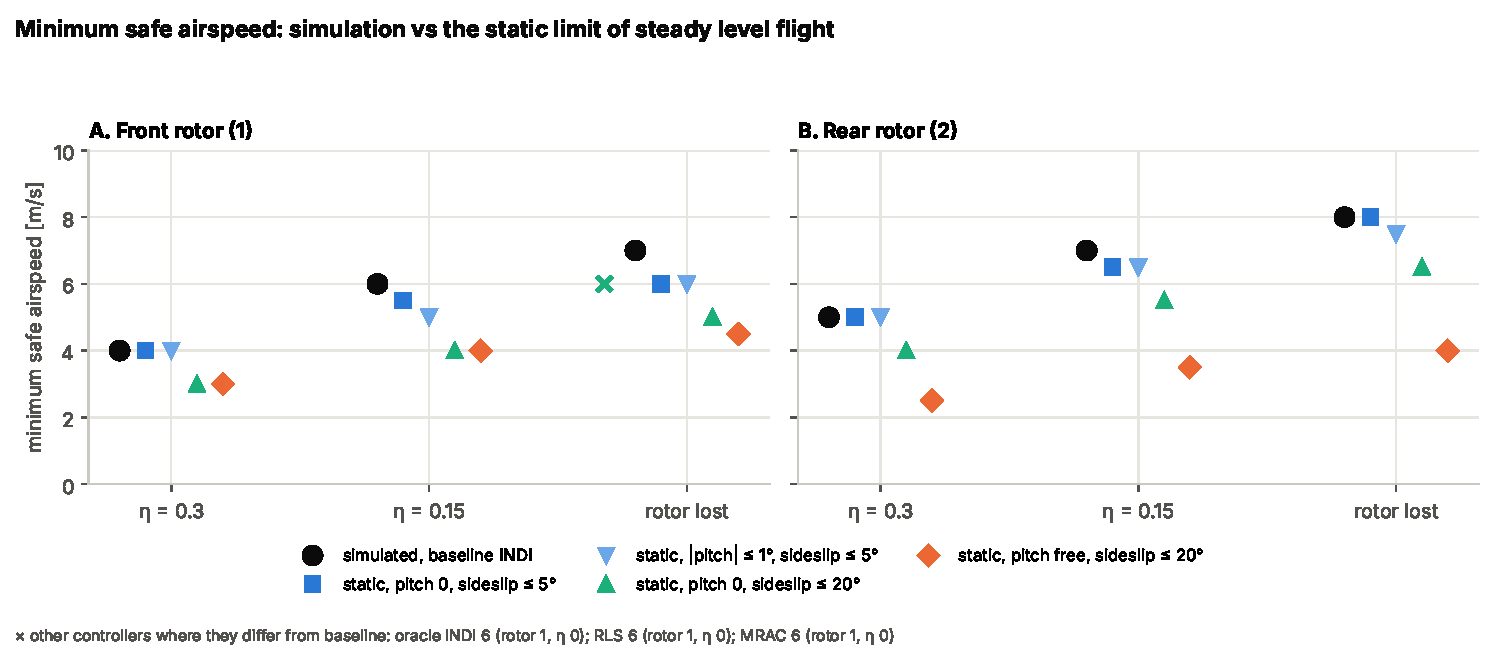
\includegraphics[width=0.85\linewidth]{fig3_min_safe_airspeed.pdf}
\caption{Minimum safe airspeed: simulation (baseline INDI) against static trim feasibility under four sets of constraints.}
\label{fig:feas}
\end{figure}

\subsection{What the estimators need}\label{sec:lockin}
\paragraph{RLS: the wing's contribution and a lower bound.} In our first quadplane runs RLS closed only 42\,\% of the gap. Two causes were
found. First, its measurement model removed only the surfaces' increment and left the wing's damping in $\vect y$, which the regression
attributed to the rotors: on noise-free data at 8\,m/s, batch least squares returned $\hat{\vect\eta} = [-0.13, -3.57, 0.46, 0.54]$ for a true
$[0.6, 1, 1, 1]$. The tuning had answered this with a dead-zone so wide that above 6\,m/s RLS made no updates at all. With the known non-rotor
part removed, the regression is unbiased. Second, with $\eta_{\min} = 0$ an abrupt fault drives all four estimates to zero within
20--50\,ms. With $\hat\eta_i = 0$ the allocation sees no effectiveness in rotor $i$ and stops moving it; without increments $\Delta u_i$ the
estimator receives no new information, and the estimate stays at zero. In one Monte Carlo case, a mild fault ($\eta = 0.59$ at 2.8\,m/s),
this gave, in the first rerun, a peak tilt of 33$^\circ$ against 0.38$^\circ$ with $\eta_{\min} = 0.1$. With the bound at 0, RLS closes 81\,\% on the grid,
$-38$\,\% in the Monte Carlo set and 20\,\% in the transition, with 6 extra losses in the speed sweep and 2 in the transition
(Table~\ref{tab:sens}). We therefore use $\eta_{\min} = 0.1$, as on the quadrotor. This choice was made after seeing the results; the cost
is that the estimate cannot show a lost rotor exactly. We expect the lock-in in any estimator that feeds an allocation which can switch an
actuator off on the basis of the estimate.

\paragraph{RLS does not identify the fault.} The bound prevents the lock-in, but not a milder form of it. After an abrupt fault the
allocation quickly redistributes the load, the increments $\Delta\vect u_f$ fall below the dead-zone within about 0.2\,s, and the estimate
freezes. Where it freezes depends on the transient, not on the fault: rotor 1 at $\eta = 0.6$ and 8\,m/s ends at
$\hat{\vect\eta} = [0.32, 0.93, 1.21, 0.83]$. The mean final estimate error is 0.15 on the grid and 0.12 in the transition, the same as
MRAC's in the transition. Control is nevertheless as good as the oracle's, because INDI needs only an effectiveness that explains what the
rotors did not deliver in the directions it is excited in, not the true one. RLS should therefore not be read as a fault-identification
method; a regression test in the repository pins this behaviour.

\paragraph{MRAC: the aerodynamic model and the air data.} Tuned without the nominal aerodynamic model, no MRAC setting satisfies the tuning
rule: its healthy-rotor estimates drift by at least 0.5 in steady flight. RLS without the model still works (88\,\% on the grid), but tunes
itself towards adapting less. With the model, MRAC depends on knowing the air velocity. With the aerodynamic coefficients of the true aircraft
off by up to $\pm30$\,\% and an unknown constant wind of up to 3\,m/s (100 Monte Carlo and 40 fault-free runs), MRAC's estimates drift by more
than 0.15 in 75\,\% of the fault-free flights (RLS 10\,\%) and its gap closed falls to 58\,\% [42, 75]; RLS keeps 106\,\% and
$\mathcal{L}_1$ 171\,\%. The wrong coefficients alone are harmless; the wind, which turns ground velocity into a wrong air velocity, is not.
RLS and MRAC receive the same wrong known part $\vect o$, but RLS regresses on increments, in which a constant bias cancels, while MRAC's
predictor uses $\vect o$ in absolute terms. The drift is not a start-up effect of the wind runs, which begin from a trim without wind: in
20\,s fault-free flights at 8\,m/s MRAC's estimates are still off by 1.0 in a crosswind and 0.28 in a headwind after 18\,s (RLS about 0).

\begin{table}[t]
\centering\small
\caption{Sensitivity analyses on the quadplane: gap closed (losses beyond the baseline's in brackets). Mismatch: true aerodynamic coefficients
$\pm30$\,\% and unknown wind up to 3\,m/s (Monte Carlo). Each variant is tuned with the same rule and procedure. MRAC without the aerodynamic
model has no admissible setting.}
\label{tab:sens}
\resizebox{\linewidth}{!}{\begin{tabular}{lcccccc}
\toprule
 & Grid & Speed sweep & Transition & Noise $\times2$ & Motor 50\,\% slower & Mismatch\\
\midrule
RLS ($\eta_{\min} = 0.1$) & 106\,\% & 96\,\% & 86\,\% (1) & 89\,\% & 97\,\% & 106\,\%\\
RLS, $\eta_{\min} = 0$ & 81\,\% & 79\,\% (6) & 20\,\% (2) & collapses (13) & 86\,\% & $-101$\,\% (5)\\
RLS, no aerodynamic model & 88\,\% & 82\,\% & 77\,\% (1) & -- & -- & 101\,\%\\
MRAC ($\eta_{\min} = 0$) & 63\,\% & 48\,\% & 78\,\% ($-3$) & 63\,\% & 61\,\% & 58\,\%\\
MRAC, $\eta_{\min} = 0.1$ & 61\,\% & 66\,\% & 82\,\% & -- & -- & --\\
$\mathcal{L}_1$ & 145\,\% (4) & 126\,\% (8) & 134\,\% (1) & 147\,\% (4) & 140\,\% (4) & 171\,\%\\
\bottomrule
\end{tabular}}
\end{table}

\subsection{Model sensitivity}
With twice the sensor noise or a true motor 50\,\% slower than the controller assumes, all three methods keep their results
(Table~\ref{tab:sens}). RLS with $\eta_{\min} = 0$ does not: with twice the noise its dead-zone no longer covers the closed-loop bias, the
estimates reach the lower bound before any fault occurs, and 15 of 72 runs are lost.

% =====================================================================================================
\section{Delay robustness}\label{sec:delay}
\begin{figure}[t]
\centering
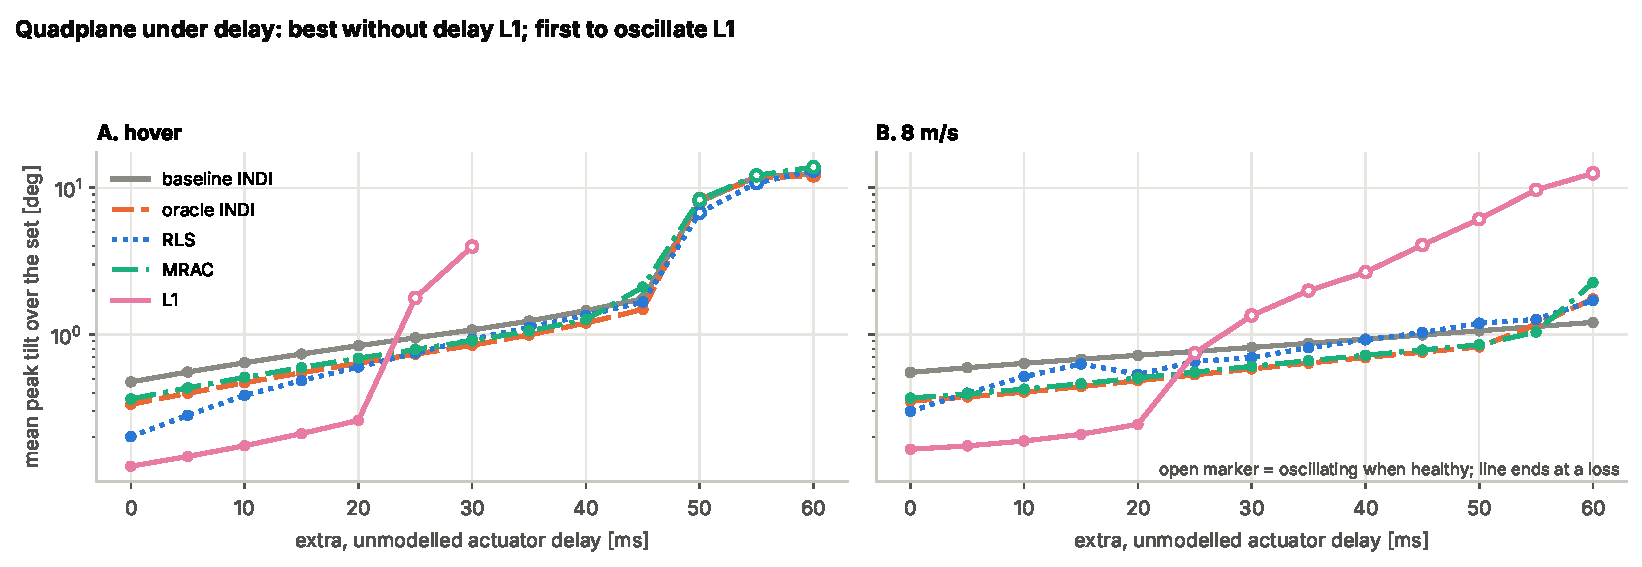
\includegraphics[width=0.9\linewidth]{fig4_delay_quadplane.pdf}
\caption{Quadplane with an unmodelled actuator delay: mean peak tilt over (A) three hover and (B) four forward-flight scenarios. Open markers:
the healthy aircraft oscillates; a line ends at a loss.}
\label{fig:delay}
\end{figure}
An unmodelled transport delay on every actuator command (Fig.~\ref{fig:delay}) leaves baseline, oracle, RLS and MRAC free of oscillation up to
25\,ms on the quadrotor, 45\,ms in hover on the quadplane and at least 60\,ms at 8\,m/s, where the wing adds damping. The tuned $\mathcal{L}_1$
oscillates from 20 and 25\,ms on both vehicles. These are oscillation-threshold margins on a 5\,ms grid. To explain this we
modelled one rotational axis exactly as implemented (motor lag, filters, INDI step, $\mathcal{L}_1$ blocks, 2\,ms sample time) and computed
the largest delay that keeps all closed-loop eigenvalues inside the unit circle (Table~\ref{tab:lin}). The model reproduces the simulated
margins: 18\,ms for the tuned $\mathcal{L}_1$ on the quadrotor, and 44\,ms (baseline) and 22\,ms ($\mathcal{L}_1$) for the quadplane in hover. Breaking the loop at the actuator command shows the mechanism: $\mathcal{L}_1$ raises the
crossover frequency of the inner loop from 3.9 to 8.0\,Hz, which is why it rejects faults and gusts faster, and the delay margin is roughly
the phase margin divided by the crossover frequency. A larger predictor pole $a$ raises the crossover less and adds phase; a narrower filter
$\omega_c$ lowers the crossover but costs phase through its own lag, so it does not help; on the quadplane $\omega_c = 320$, 640 and 1280\,rad/s
all give about 20\,ms. The model has no surfaces or aerodynamic damping and is valid only in hover; at 8\,m/s the simulated baseline does
not oscillate up to 60\,ms.

\begin{table}[t]
\centering\small
\caption{One-axis linear analysis (quadrotor roll axis). Delay margin from the closed-loop eigenvalues; simulation in brackets.}
\label{tab:lin}
\begin{tabular}{lccc}
\toprule
 & Crossover & Phase margin & Delay margin\\
\midrule
Baseline INDI & 3.85\,Hz & 44.2$^\circ$ & 30\,ms (25)\\
$\mathcal{L}_1$, $a = 0.1$, $\omega_c = 1280$ (tuned) & 7.97\,Hz & 54.2$^\circ$ & 18\,ms (18)\\
$\mathcal{L}_1$, $a = 100$, $\omega_c = 1280$ & 7.38\,Hz & 60.1$^\circ$ & 22\,ms (22)\\
$\mathcal{L}_1$, $a = 300$, $\omega_c = 1280$ & 6.07\,Hz & 66.6$^\circ$ & 30\,ms (25)\\
$\mathcal{L}_1$, $a = 10$, $\omega_c = 320$ (first tuning) & 7.57\,Hz & 50.1$^\circ$ & 18\,ms (18)\\
\bottomrule
\end{tabular}
\end{table}

% =====================================================================================================
\section{Faults during the transition}
\begin{figure}[t]
\centering
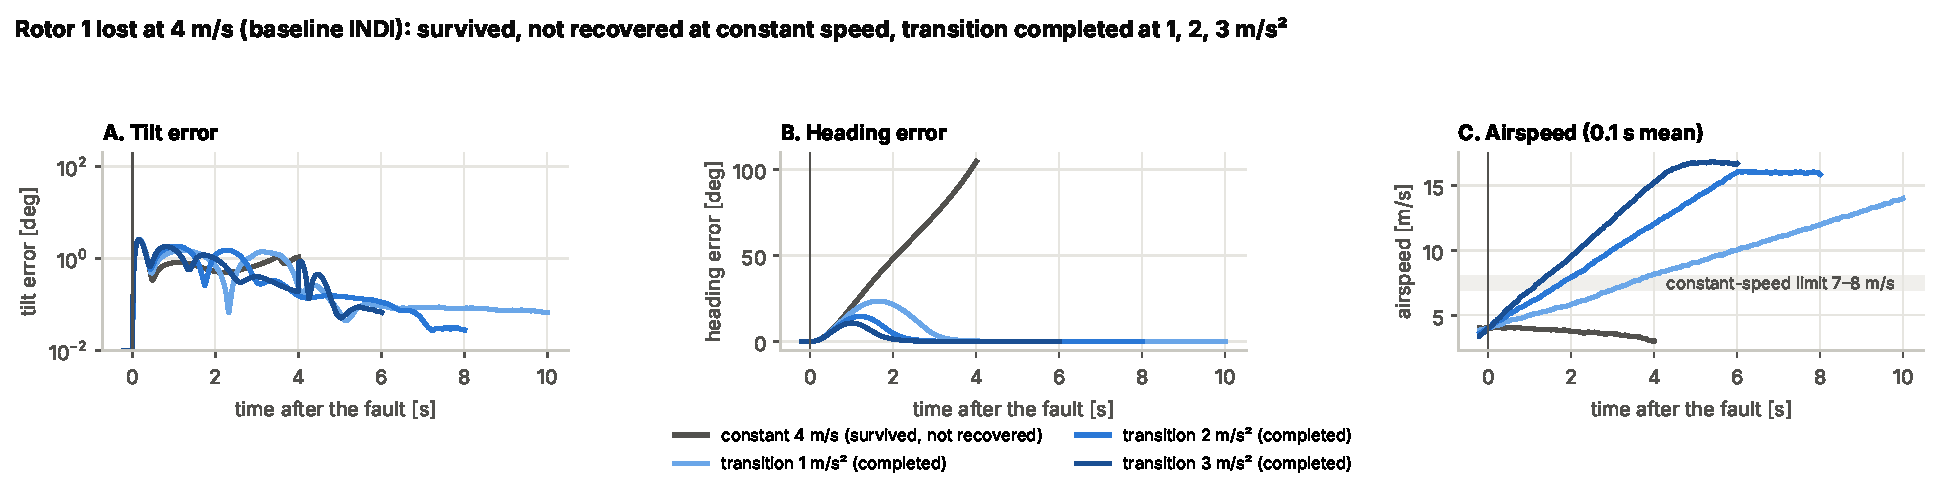
\includegraphics[width=\linewidth]{fig6_transition_outrun.pdf}
\caption{Rotor 1 lost at 4\,m/s, baseline INDI. At constant speed the aircraft stays upright but loses heading; during a transition at
1, 2 or 3\,m/s$^2$ it reaches the safe speed band, recovers the heading and completes the transition.}
\label{fig:trans}
\end{figure}
During the transition the airspeed is not constant, so the limit of the previous section moves while the fault develops. The aircraft
starts in hover and accelerates at 1, 2 or 3\,m/s$^2$ to 16\,m/s; with the controllers' settings unchanged, a front or rear rotor fails as
the reference passes $V_f$. A run is \emph{completed} if it recovers and ends within 1\,m/s of cruise speed. After a complete rotor loss the
transition is completed from $V_f = 4$\,m/s for the front rotor at every acceleration and for the rear rotor from 2, 4 and 6\,m/s at 1,
2 and 3\,m/s$^2$, against 6--7 / 8\,m/s at constant speed; for
$\eta = 0.3$ from 0--2\,m/s against 4 / 5\,m/s (Fig.~\ref{fig:trans}). The vehicle needs a few seconds to lose its heading after the loss;
if it reaches the safe band within that time, the surfaces take over. The boundary is the same for every controller, except
$\mathcal{L}_1$ with the rear rotor lost at 1\,m/s$^2$ (4\,m/s); the criteria differ (completed is judged at the end of the transition,
recovered in a 4\,s window). The ranking of the methods is unchanged: gap closed $\mathcal{L}_1$ 134\,\% [127, 141], RLS 86\,\% [80, 93],
MRAC 78\,\% [64, 91] (83\,\% on the common set). The baseline loses 7 of 84 runs, RLS and $\mathcal{L}_1$ 8 and MRAC 4: in three complete
losses at $V_f \le 2$\,m/s MRAC survives without completing where the baseline is lost. RLS with $\eta_{\min} = 0$ reaches 20\,\% with 9 losses.

% =====================================================================================================
\section{Discussion}
\begin{figure}[t]
\centering
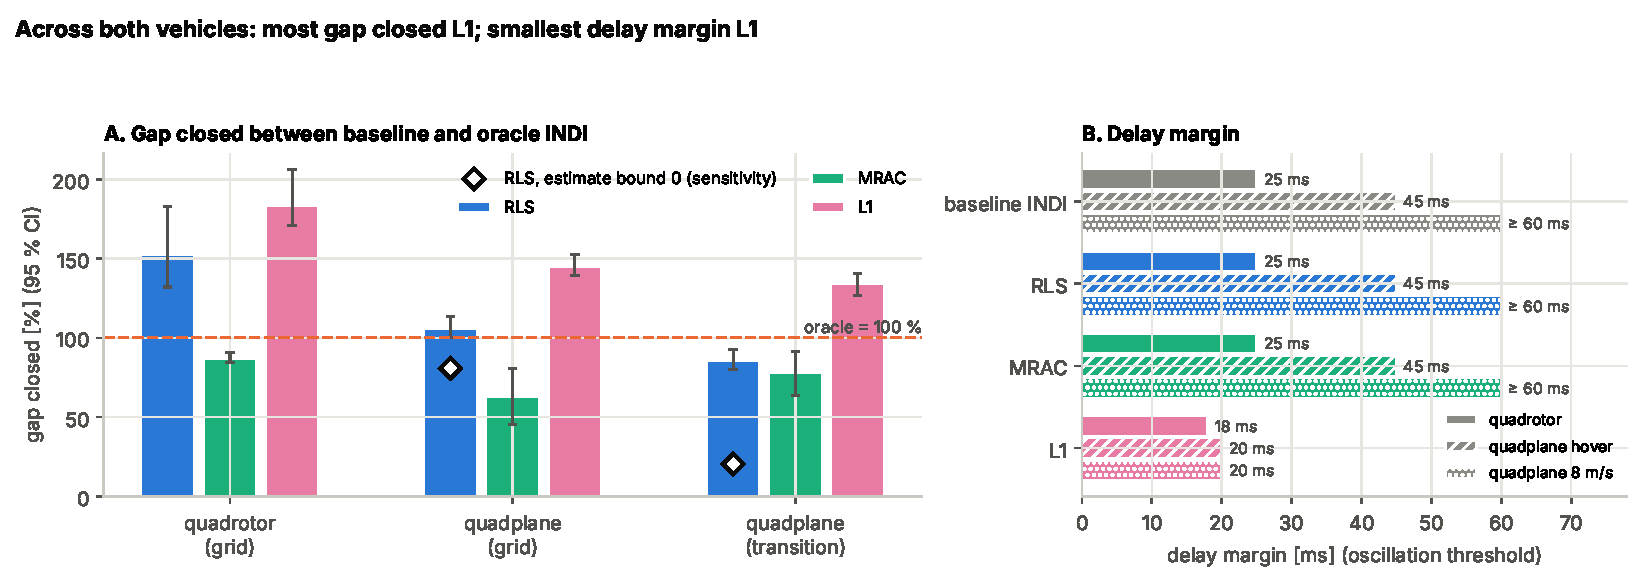
\includegraphics[width=\linewidth]{fig5_summary.pdf}
\caption{Both vehicles at a glance. (A) Gap closed with 95\,\% intervals; open diamonds: RLS with $\eta_{\min} = 0$ (sensitivity). (B) Delay margin
(quadrotor; quadplane in hover; quadplane at 8\,m/s).}
\label{fig:summary}
\end{figure}
\paragraph{Which method?} Figure~\ref{fig:summary} summarises both vehicles. $\mathcal{L}_1$ recovers fastest on both vehicles, handles gusts correctly and is insensitive to noise and motor
mismatch, but its gain in bandwidth costs delay margin; on a real aircraft the predictor pole should be chosen from the expected delay,
not from a delay-free simulation. RLS reaches the oracle on both vehicles when its measurement model is complete and its estimate is bounded
away from zero, but it does not identify the fault and it reacts to gusts as if they were faults. MRAC is never the fastest but loses the
fewest runs in the transition; on the quadplane it rests on
the aerodynamic model and on air data, and an unknown wind is enough to corrupt its estimates.

\paragraph{Fair comparison.} Several of our own first readings did not survive checking: that RLS is weak on the quadplane because of
its inertia (it was an incomplete measurement model and the lock-in), that RLS identifies the fault (it controls well with a wrong
estimate), that $\mathcal{L}_1$ gains most at low airspeed (an artefact of the first wing model), and that the minimum airspeed is physical
without qualification (it is, under pitch and heading hold). Some were caught by questions the benchmark could not answer itself, a trace of
the worst case and a controller-independent trim analysis; the others by two independent reviews of the code. The outcome of a complete
rotor loss in hover changed twice with corrections of the aerodynamic model at large angles; we therefore report only that no controller
recovers it. The reviews also showed that the RLS bound is a design decision with a large effect, and we report both values.

\paragraph{Limitations.} Simulation only; parameters from a public model and a textbook aircraft, not an identified vehicle. No rotor--wing
interaction and no rotor drag (hence no yaw damping in hover); rotor thrust independent of airspeed; no rudder; the post-stall moments are a
simple flat-plate model, and the surface and damping derivatives are not reduced beyond stall. Position, velocity and attitude are measured
without noise; only the gyroscope, accelerometer and pitot are noisy. The RLS bound on the quadplane was changed after seeing results. MRAC
and RLS use the nominal aerodynamics and treat ground velocity as air velocity. The tuning gives every method the same procedure and
budget, but not the same resolution per parameter. Bibliographic and literature checks rely partly on abstracts.

% =====================================================================================================
\section{Conclusion}
Under one protocol on two vehicles, $\mathcal{L}_1$ augmentation of INDI recovers fastest from rotor faults and gusts and keeps doing so
with doubled noise and a slower motor, at the cost of the smallest delay margin, which a one-axis linear model explains through the raised
inner-loop crossover. Estimation-based adaptation by RLS reaches the oracle when its measurement model includes the wing and its estimate
cannot reach zero, where it would lock itself out of an over-actuated allocation, although its estimate then freezes at a wrong value and
does not identify the fault; MRAC needs the aerodynamic model and correct air data. On a
quadplane, a lift-rotor loss is recoverable from 6--8\,m/s at constant speed, a physical limit under pitch and heading hold, and continuing the
transition lets the aircraft outrun a loss at 4\,m/s (rear rotor at 1\,m/s$^2$: 2\,m/s). Next steps are a recovery mode that uses sideslip and pitch, delay-aware
tuning of $\mathcal{L}_1$, and validation in PX4 software-in-the-loop simulation.

% =====================================================================================================
\begin{thebibliography}{99}\small
\bibitem{sieberling2010} S.~Sieberling, Q.~P.~Chu, J.~A.~Mulder, ``Robust flight control using incremental nonlinear dynamic inversion and angular acceleration prediction,'' \emph{Journal of Guidance, Control, and Dynamics}, vol.~33, no.~6, pp.~1732--1742, 2010, doi:10.2514/1.49978.
\bibitem{smeur2016} E.~J.~J.~Smeur, Q.~P.~Chu, G.~C.~H.~E.~de Croon, ``Adaptive incremental nonlinear dynamic inversion for attitude control of micro air vehicles,'' \emph{Journal of Guidance, Control, and Dynamics}, vol.~39, no.~3, pp.~450--461, 2016, doi:10.2514/1.G001490.
\bibitem{sun2020} S.~Sun, X.~Wang, Q.~P.~Chu, C.~C.~de Visser, ``Incremental nonlinear fault-tolerant control of a quadrotor with complete loss of two opposing rotors,'' \emph{IEEE Transactions on Robotics}, vol.~37, no.~1, pp.~116--130, 2021, doi:10.1109/TRO.2020.3010626.
\bibitem{deponti2023} T.~M.~L.~De Ponti, E.~J.~J.~Smeur, B.~W.~D.~Remes, ``Incremental nonlinear dynamic inversion controller for a variable skew quad plane,'' in \emph{International Conference on Unmanned Aircraft Systems (ICUAS)}, pp.~241--248, 2023, doi:10.1109/ICUAS57906.2023.10156289.
\bibitem{falconi2021} G.~P.~Falcon\'{\i} Salazar, \emph{Adaptive Fault Tolerant Control for VTOL Aircraft with Actuator Redundancy}, thesis, Technical University of Munich, TUM.University Press, 2022, ISBN 978-3-95884-074-4.
\bibitem{franceschini2026} G.~Franceschini, G.~Raos, G.~Gozzini, D.~Invernizzi, ``Adaptive control allocation for incremental nonlinear dynamic inversion under actuator degradation,'' in \emph{34th Mediterranean Conference on Control and Automation (MED)}, pp.~704--709, 2026, doi:10.1109/MED70602.2026.11598288.
\bibitem{hovakimyan2010} N.~Hovakimyan, C.~Cao, \emph{$\mathcal{L}_1$ Adaptive Control Theory: Guaranteed Robustness with Fast Adaptation}, SIAM, 2010.
\bibitem{raos2026} G.~Raos, G.~Gozzini, D.~Invernizzi, ``Performance and robustness analysis of INDI flight control laws with $\mathcal{L}_1$ adaptive augmentation,'' CEAS EuroGNC, paper CEAS-GNC-2026-072, 2026.
\bibitem{mao2023} J.~Mao, J.~Yeom, S.~Nair, G.~Loianno, ``From propeller damage estimation and adaptation to fault tolerant control: enhancing quadrotor resilience,'' \emph{IEEE Robotics and Automation Letters}, 2024, doi:10.1109/LRA.2024.3380923 (arXiv:2310.13091).
\bibitem{wang2021} X.~Wang, S.~Sun, ``Incremental fault-tolerant control for a hybrid quad-plane UAV subjected to a complete rotor loss,'' \emph{Aerospace Science and Technology}, vol.~125, 107105, 2022, doi:10.1016/j.ast.2021.107105.
\bibitem{cai2025} J.~Cai, M.~Lovera, ``An active fault-tolerant online control allocation scheme for a dual-system UAV in transition flight,'' arXiv:2510.04853, 2025.
\bibitem{fu2025} Y.~Fu, B.~Wang, H.~Zhao, M.~Zhou, N.~Li, Z.~Gao, ``Adaptive safety attitude control of a hybrid VTOL UAV under transition flight subject to multiple faults and uncertainties,'' \emph{Aerospace Science and Technology}, vol.~163, 110284, 2025.
\bibitem{mueller2014} M.~W.~Mueller, R.~D'Andrea, ``Stability and control of a quadrocopter despite the complete loss of one, two, or three propellers,'' in \emph{IEEE International Conference on Robotics and Automation (ICRA)}, pp.~45--52, 2014, doi:10.1109/ICRA.2014.6906588.
\bibitem{harkegard2002} O.~H\"{a}rkeg\aa{}rd, ``Efficient active set algorithms for solving constrained least squares problems in aircraft control allocation,'' in \emph{41st IEEE Conference on Decision and Control}, vol.~2, pp.~1295ff., 2002, doi:10.1109/CDC.2002.1184694.
\bibitem{beard2012} R.~W.~Beard, T.~W.~McLain, \emph{Small Unmanned Aircraft: Theory and Practice}, Princeton University Press, 2012; coefficients from \texttt{github.com/byu-magicc/mavsim\_public}.
\bibitem{px4models} PX4 Gazebo models, \texttt{standard\_vtol}, \texttt{github.com/PX4/PX4-gazebo-models}, accessed 27 Oct 2026.
\end{thebibliography}
\end{document}
